\documentclass[14pt]{beamer}

\usepackage{graphicx}
\usepackage{amsmath}
\usepackage{moresize}
\usepackage[normalem]{ulem}

\renewcommand<>{\sout}[1]{
  \alt#2{\beameroriginal{\sout}{#1}}{#1}
}

\usetheme{Boadilla}
\usecolortheme{beaver}
\beamertemplatenavigationsymbolsempty
\setlength{\parskip}{1em}

% http://rkd.zgib.net/wiki/DebianBeamerThemes
\definecolor{debianred}{rgb}{.780,.000,.211} % 199,0,54
\definecolor{debianblue}{rgb}{0,.208,.780} % 0,53,199
\definecolor{debianlightbackgroundblue}{rgb}{.941,.941,.957} % 240,240,244
\definecolor{debianbackgroundblue}{rgb}{.776,.784,.878} % 198,200,224
\usecolortheme[named=debianbackgroundblue]{structure}
\setbeamercolor{normal text}{fg=debianred}
\setbeamercolor{titlelike}{parent=none,fg=debianblue}
\setbeamercolor{sidebar}{fg=debianred,bg=debianbackgroundblue}
\setbeamercolor{palette sidebar primary}{fg=debianred}
\setbeamercolor{palette sidebar secondary}{fg=debianred}
\setbeamercolor{palette sidebar tertiary}{fg=debianred}
\setbeamercolor{palette sidebar quaternary}{fg=debianred}
\setbeamercolor{section in toc}{fg=debianred}
\setbeamercolor{subsection in toc}{parent=debianred}
\setbeamercolor{item}{fg=debianred}
\setbeamercolor{block title}{fg=debianblue}

\logo{
\includegraphics[viewport=274 335 360 440,width=1cm]{openlogo-nd}}
\title[Debian]{
\includegraphics[viewport=274 335 360 440,height=3.5cm]{openlogo}}
\author[Corey Ford]{Corey Ford\\(\texttt{coyotebush})\vspace{-2em}}
\institute[CPLUG]{CPLUG\vspace{-2em}}
\date{2014-10-09}

\begin{document}

\frame[plain]{\titlepage}

\section{History}

\begin{frame}
  \frametitle{My history}

  Grew up on OS X

  Linux in VMs for fun (Fedora, Arch, Debian\ldots)

  Got ThinkPad, installed Debian

\end{frame}

\begin{frame}
  \frametitle{Debian history}

  1993: Ian Murdock

  1990s: Grew up

  1999: First derivatives

  2000: Knoppix

  2004: Ubuntu

\end{frame}

\section{Philosophy}

\begin{frame}
  \frametitle{Debian philosophy}

  Open development
  (Debian Social Contract)

  Free software*
  (Debian Free Software Guidelines)

  Democracy
  (Debian Constitution)

\end{frame}

\begin{frame}
  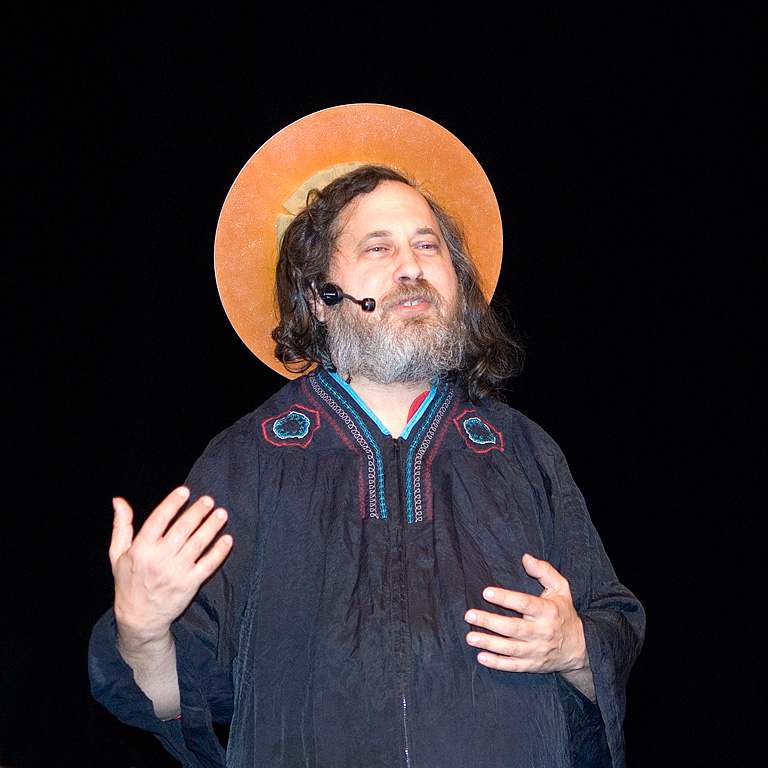
\includegraphics{rms}
\end{frame}

\begin{frame}[fragile]
\scriptsize
\begin{verbatim}
$ vrms
              Non-free packages installed on gwaihir

firmware-iwlwifi                    Binary firmware for Intel Wireless cards
firmware-linux                      Binary firmware for various drivers in the Linux kerne
firmware-linux-nonfree              Binary firmware for various drivers in the Linux kerne
intel-microcode                     Processor microcode firmware for Intel CPUs
skype                               Wherever you are, wherever they are
virtualbox-guest-additions-iso      guest additions iso image for VirtualBox

               Contrib packages installed on gwaihir

flashplugin-nonfree                 Adobe Flash Player - browser plugin
iucode-tool                         Intel processor microcode tool
ttf-mscorefonts-installer           Installer for Microsoft TrueType core fonts
virtualbox                          x86 virtualization solution - base binaries
virtualbox-dkms                     x86 virtualization solution - kernel module sources fo
virtualbox-qt                       x86 virtualization solution - Qt based user interface

  6 non-free packages, 0.3% of 2235 installed packages.
  6 contrib packages, 0.3% of 2235 installed packages.
\end{verbatim}
\end{frame}


\begin{frame}
  \frametitle{``The Universal Operating System''}

  Architectures: 13 official, 10+ unofficial

  Kernels: Linux, FreeBSD, Hurd?

  Packages: 37,500+

\end{frame}

\begin{frame}
  \frametitle{Debian releases}

  \begin{align*}
    &\ldots\\
    &\mathtt{lenny}\\
    &\mathtt{squeeze}\\
    \mathtt{stable} \to\ &\mathtt{wheezy}\\
    \mathtt{testing} \to\ &\mathtt{jessie}\\
    \mathtt{unstable} =\ &\mathtt{sid}
  \end{align*}
\end{frame}

\section{Package management}

\begin{frame}
  \frametitle{Debian package management layers}

  dpkg (\texttt{.deb} files)

  apt (dependencies)

  frontends

\end{frame}

\begin{frame}
  \frametitle{Debian package management}

  \sout<2>{\texttt{\$ apt-get remove emacs}\\
    \texttt{\$ apt-get install vim-gtk}}

  \invisible<1>{\texttt{\$ aptitude remove emacs}\\
    \texttt{\$ aptitude install vim-gtk}}
\end{frame}

\begin{frame}
  \texttt{\$ aptitude}

  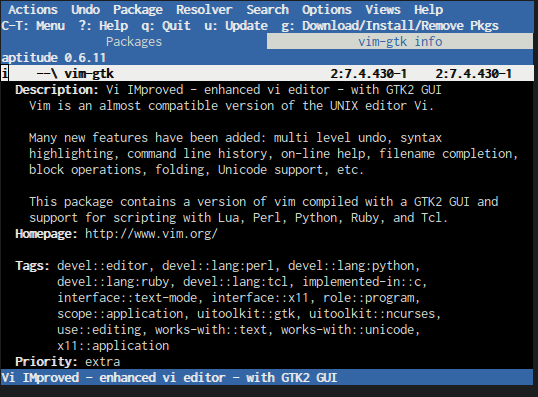
\includegraphics[height=7cm]{aptitude}
\end{frame}

\begin{frame}[fragile]
\begin{verbatim}
$ apt-get moo
                 (__) 
                 (oo) 
           /------\/ 
          / |    ||   
         *  /\---/\ 
            ~~   ~~   
..."Have you mooed today?"...
$ aptitude moo
There are no Easter Eggs in this program.
\end{verbatim}
\end{frame}

\begin{frame}[fragile]
\begin{verbatim}
$ aptitude update
$ aptitude upgrade
$ dpkg -i skype.deb
$ dpkg -L vim-gtk
$ dpkg -S /etc/vim/vimrc
\end{verbatim}
\end{frame}

\begin{frame}[fragile]
\begin{verbatim}
$ cowsay "Questions?"
 ____________
< Questions? >
 ------------
        \   ^__^
         \  (oo)\_______
            (__)\       )\/\
                ||----w |
                ||     ||
\end{verbatim}
\end{frame}

\end{document}
